As we are focusing on UC system, we do not need to consider location of university as a secondary variable. Also, we assume similar living cost in California state. Further, we do not consider ranks of university as a factor, since ranking of university are done by different agencies and we cannot ascertain their accurracy. So, our model is as follows,
\begin{equation}
  \label{eqnourmodel}
  salary = \beta_0 + \beta_1 \text{Years Since Ph.~D.} + \beta_2 \text{Productivity}
\end{equation}

\subsubsection{Years since Ph.~D.}

We looked at our data~\secref{sectionData} to see if years since Ph.~D. is a major factor to be considered for regression. So, we plotted base salary versus years since Ph.~D. From the ~\figref{figYearPhD} we see that there a strong correlation between base salary and seniority. Thus, we consider years since Ph.~D. as a secondary variable.

\begin{figure}[h]
\label{figYearPhD}
\centering
%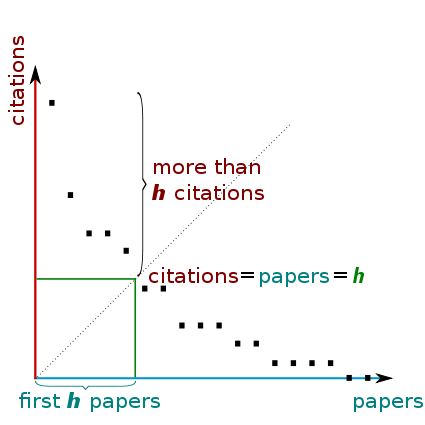
\epsfig{file=figures/hindex.eps}
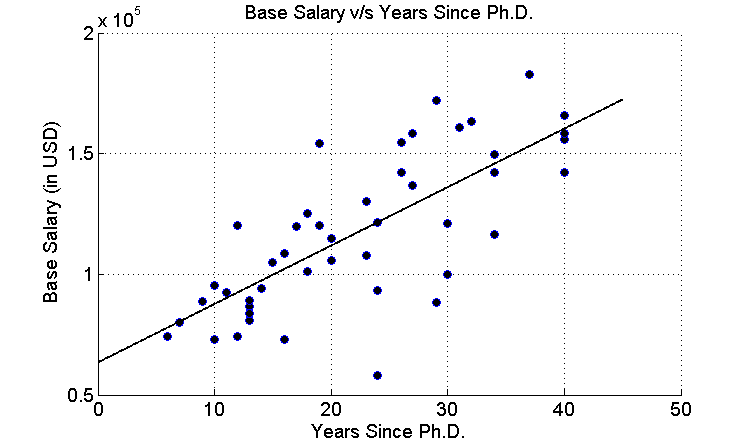
\includegraphics[width=0.5\textwidth]{figures/yrPhD.png}
\caption{Plot of base salary versus years since Ph.~D. showing correlation.}
\end{figure}
